\section{Results} % 6.4
\subsection{Results and Analysis} %6.4.1

All the acceptable results can be seen as Figure~\ref{6_4_i}. Compared to Figure~\ref{5_4_1_i}, we can see there are less acceptable tuning results in the emergency control.\\

Separately, when delay is 0.01 seconds, as shown in Figure~\ref{6_4_i} and in Figure~\ref{6_4_copare_01}, there are only four acceptable results for the emergency control. Besides, emergency control removes high-kp values to make sure the overshoot is in the set range.

Comparing Figure~\ref{6_4_CompaPlots_01}, Figure~\ref{6_4_CompaPlots_11} and Figure~\ref{6_4_CompaPlots_21}, the system is more unstable when the time delay increases.

\begin{figure}[htbp]
\centering
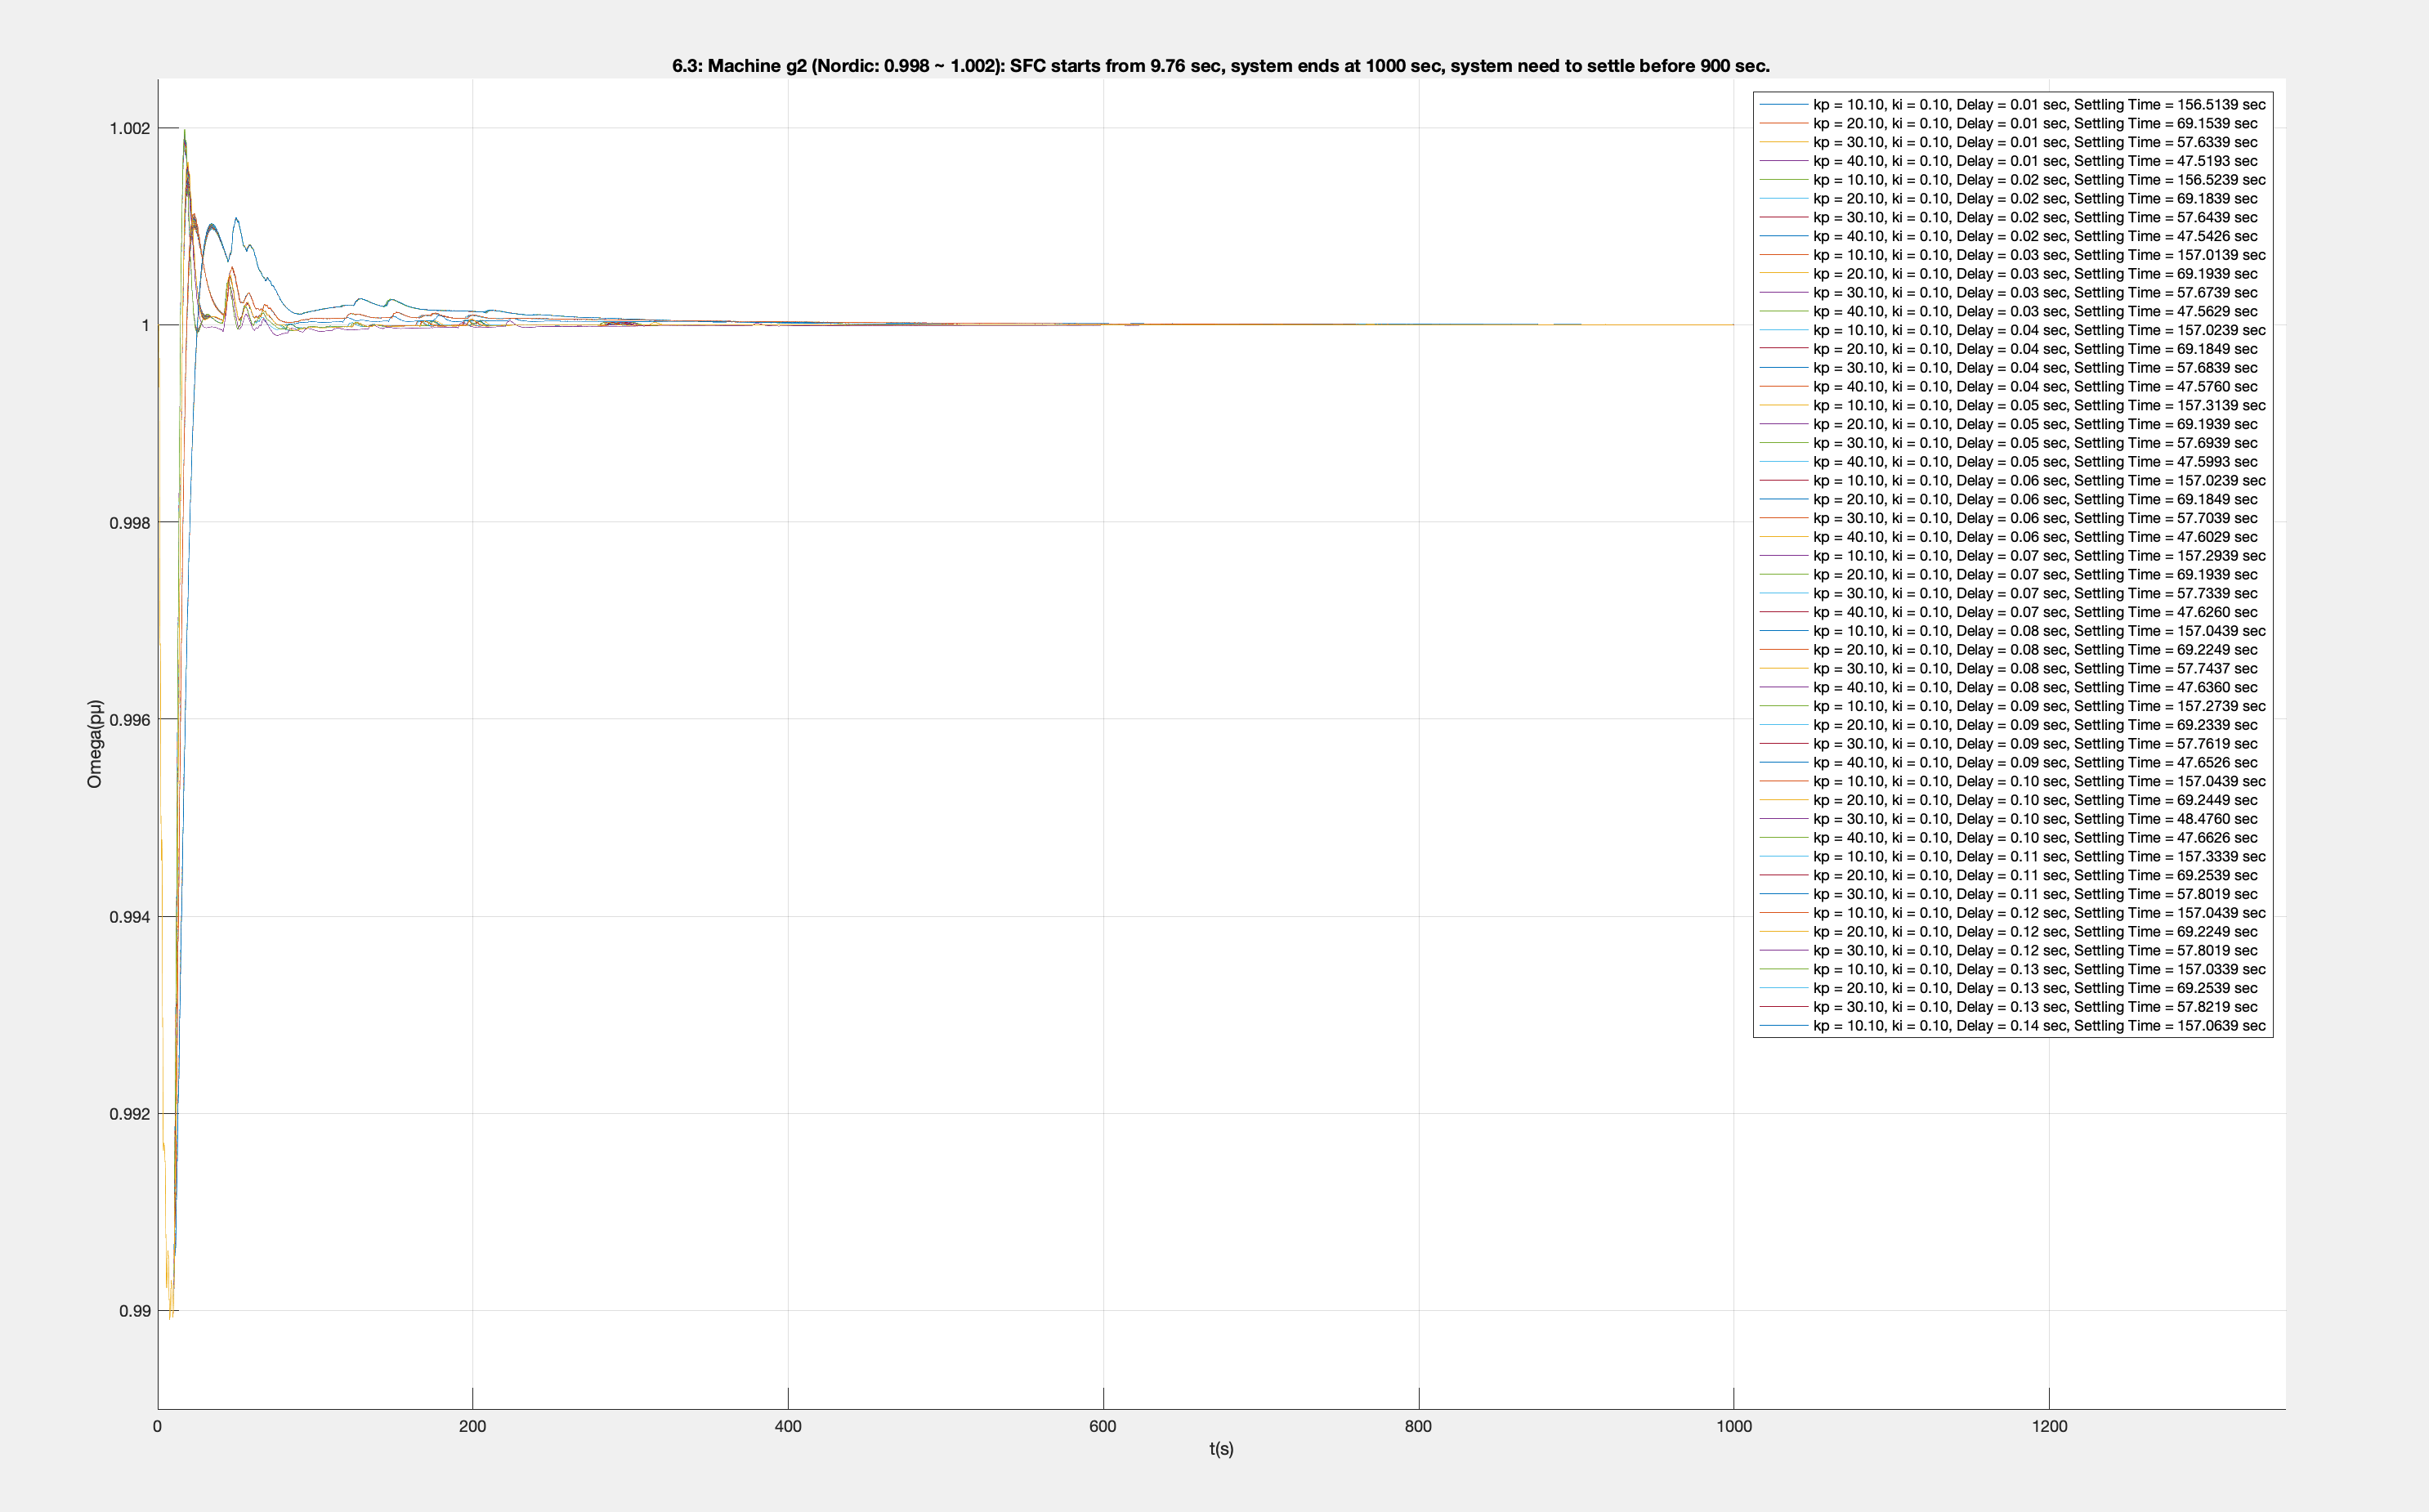
\includegraphics[width = .891\textwidth]{figure/6_4_i.png}
\caption{Acceptable results of Emergency Control.}
\label{6_4_i}
\end{figure}

\begin{figure}[htbp]
\centering
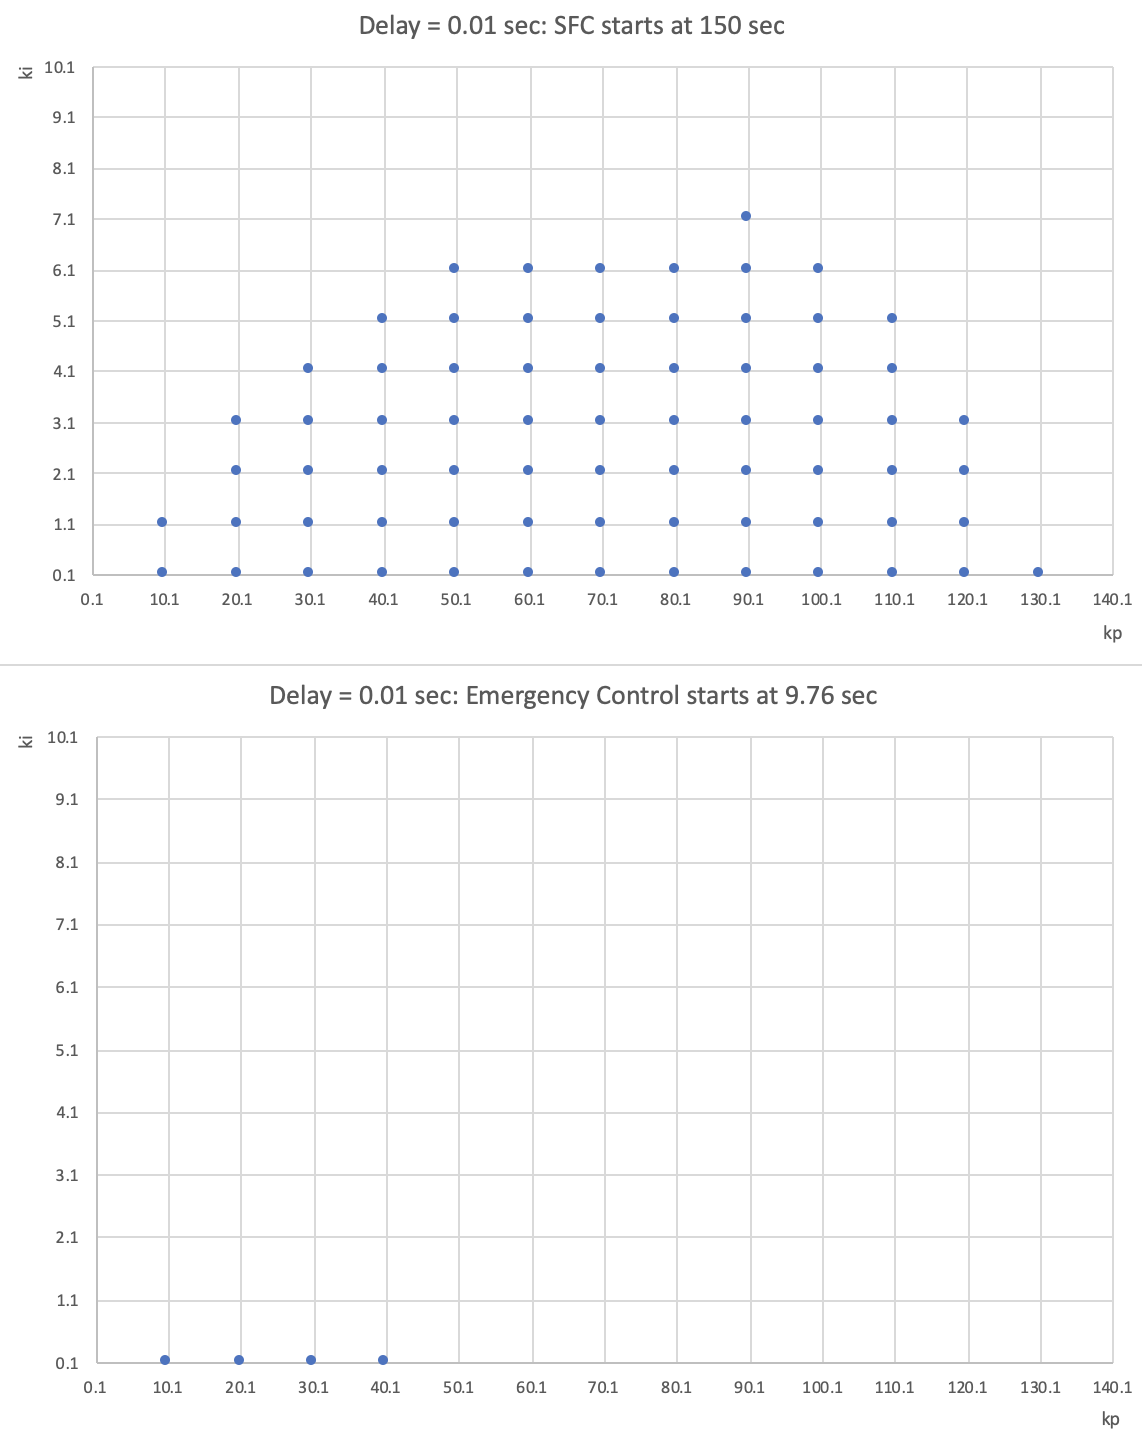
\includegraphics[width = .891\textwidth]{figure/6_4_copare_01.png}
\caption{Comparison: Delay is 0.01 sec}
\label{6_4_copare_01}
\end{figure}

\begin{figure}[htbp]
\centering
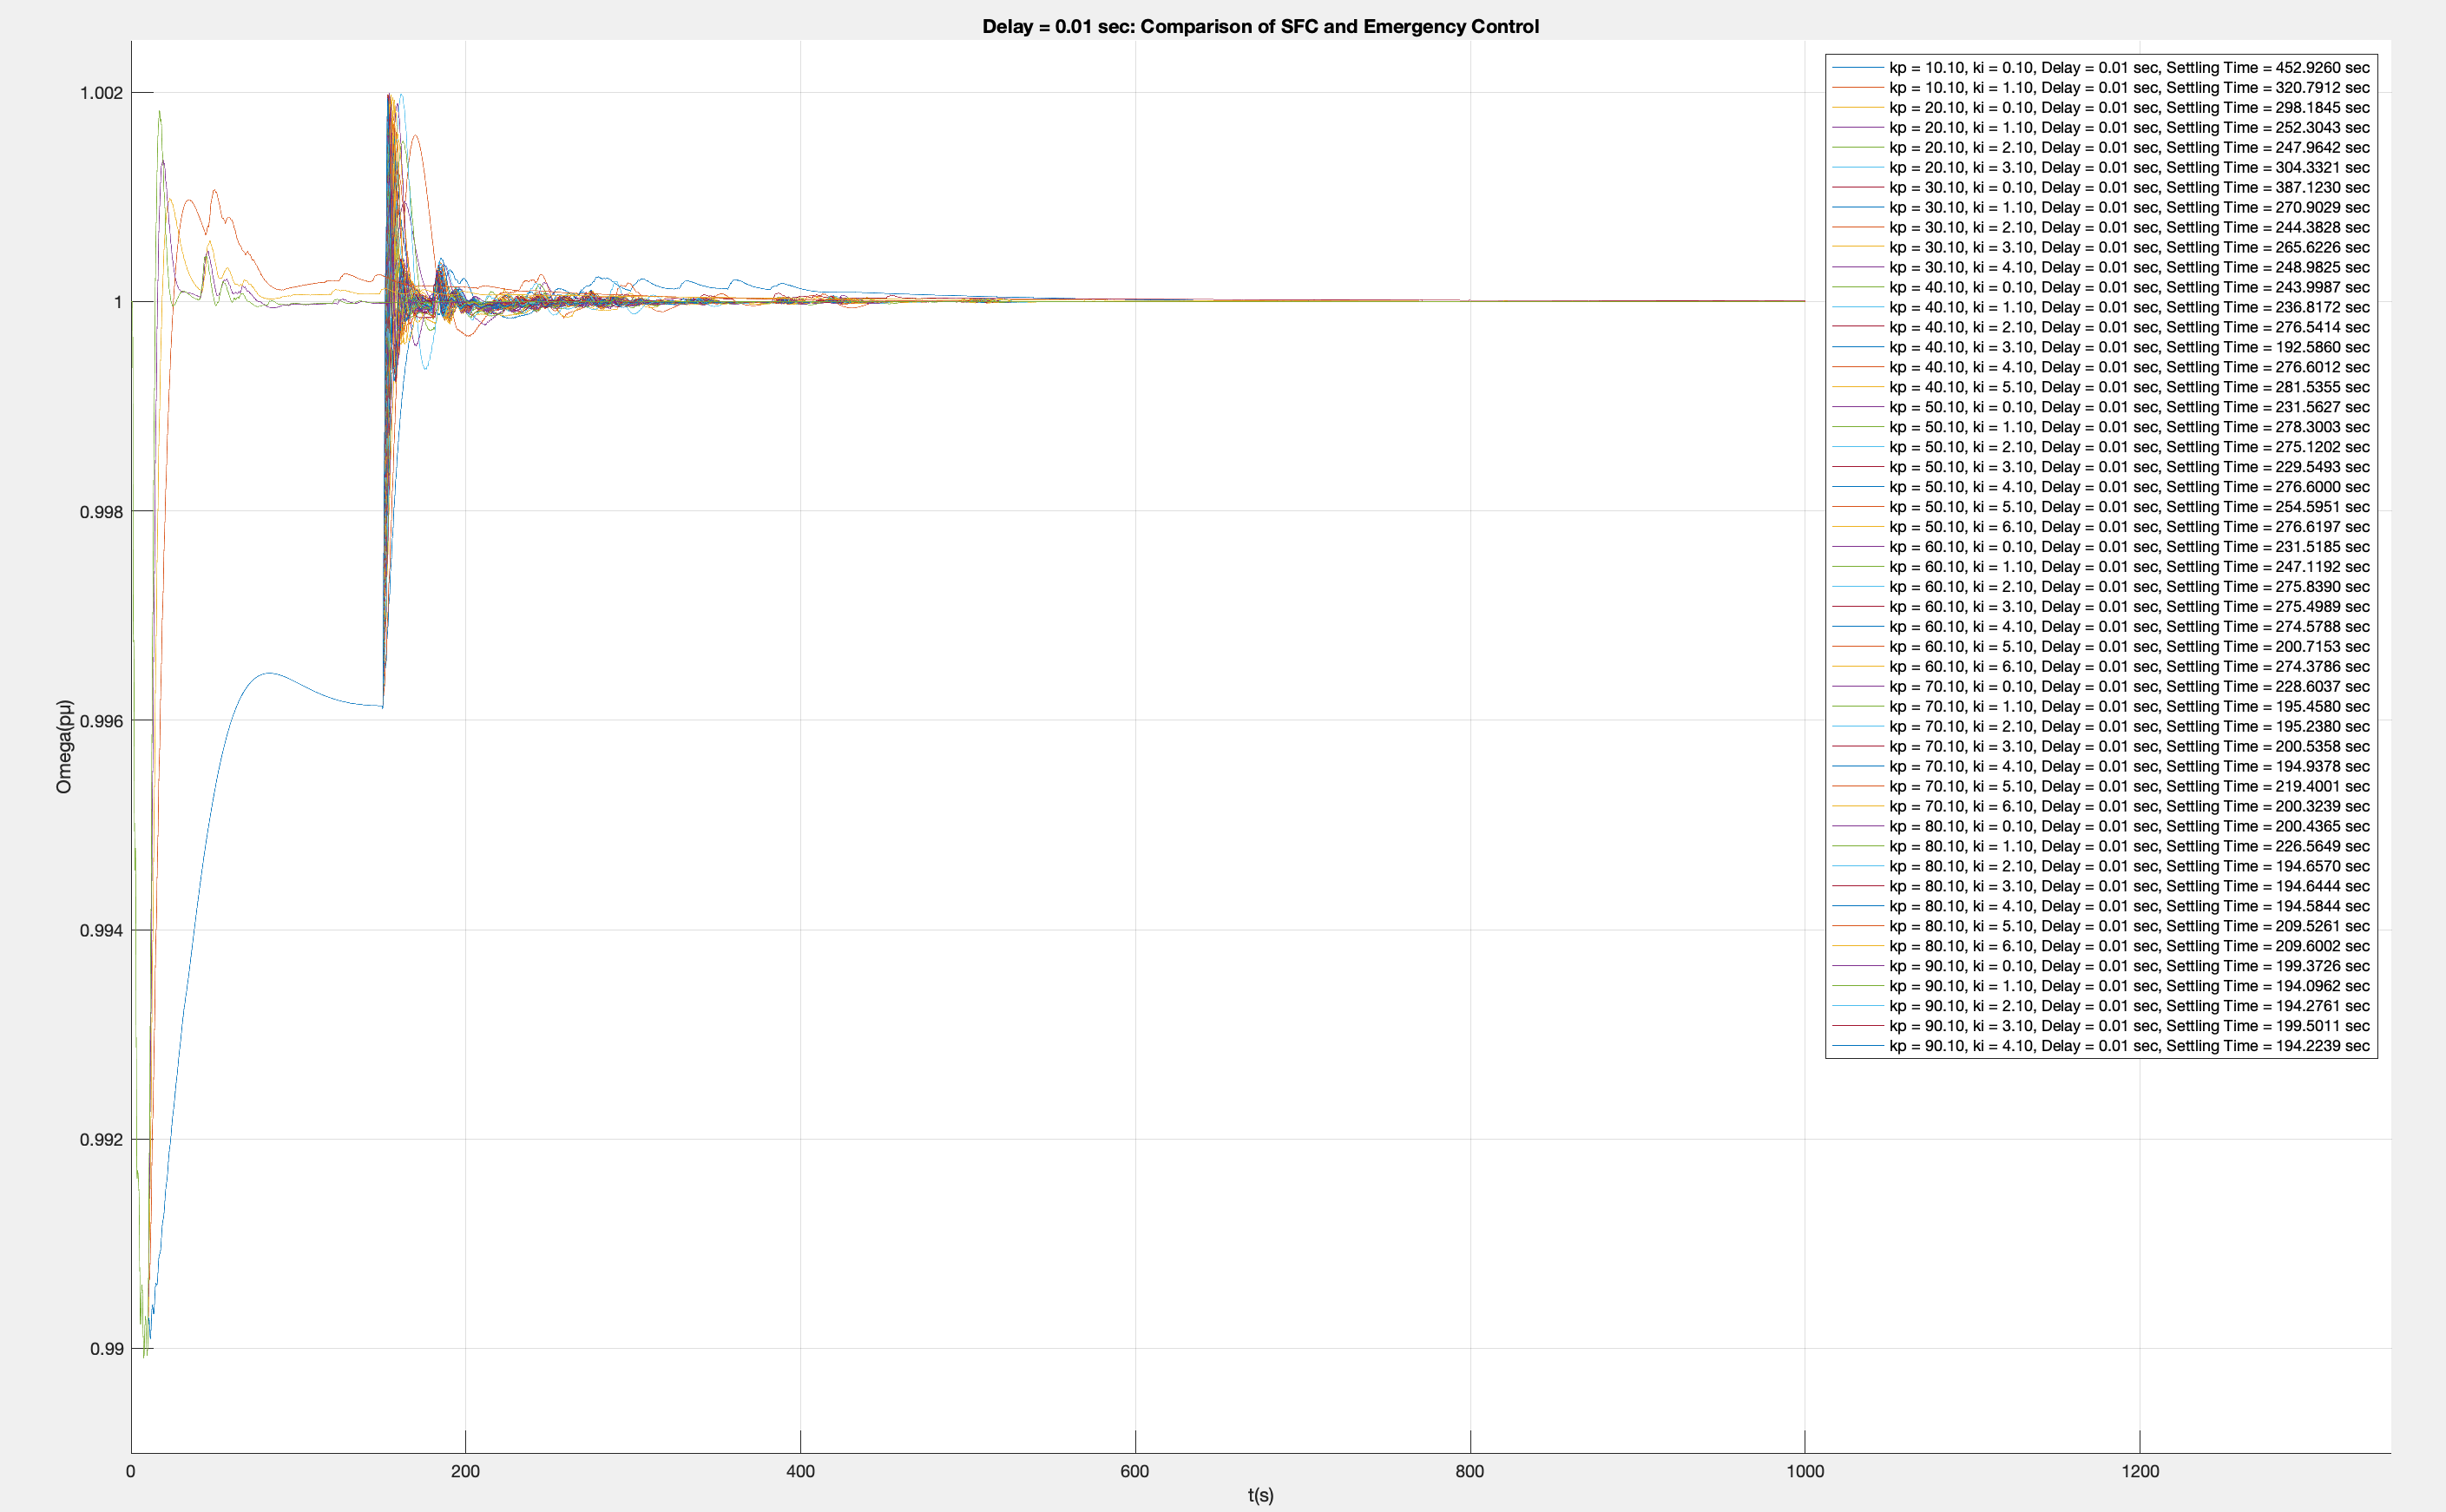
\includegraphics[width = .891\textwidth]{figure/6_4_CompaPlots_01.png}
\caption{Sketches for SFC and Emergency Control: Delay is 0.01 sec}
\label{6_4_CompaPlots_01}
\end{figure}


\begin{figure}[htbp]
\centering
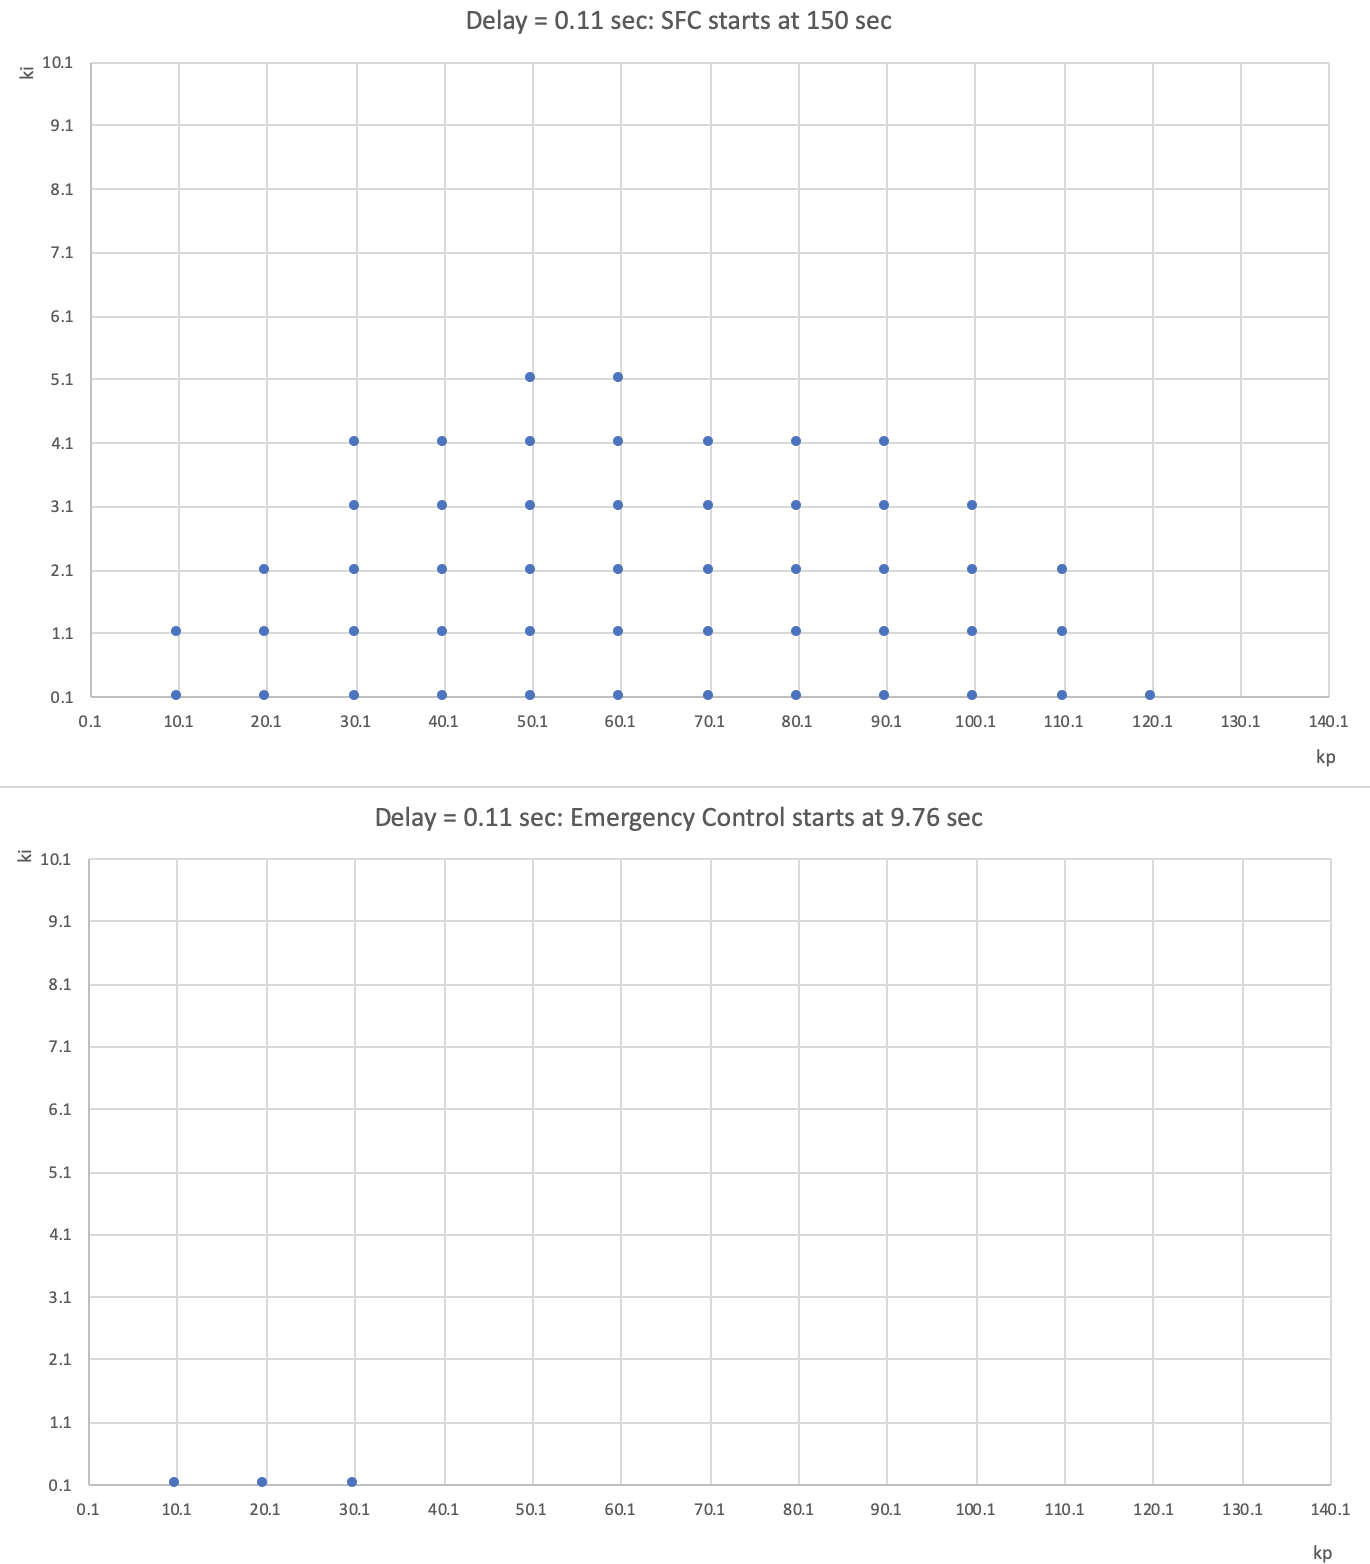
\includegraphics[width = .891\textwidth]{figure/6_4_copare_11.png}
\caption{Comparison: Delay is 0.11 sec}
\label{6_4_copare_11}
\end{figure}


\begin{figure}[htbp]
\centering
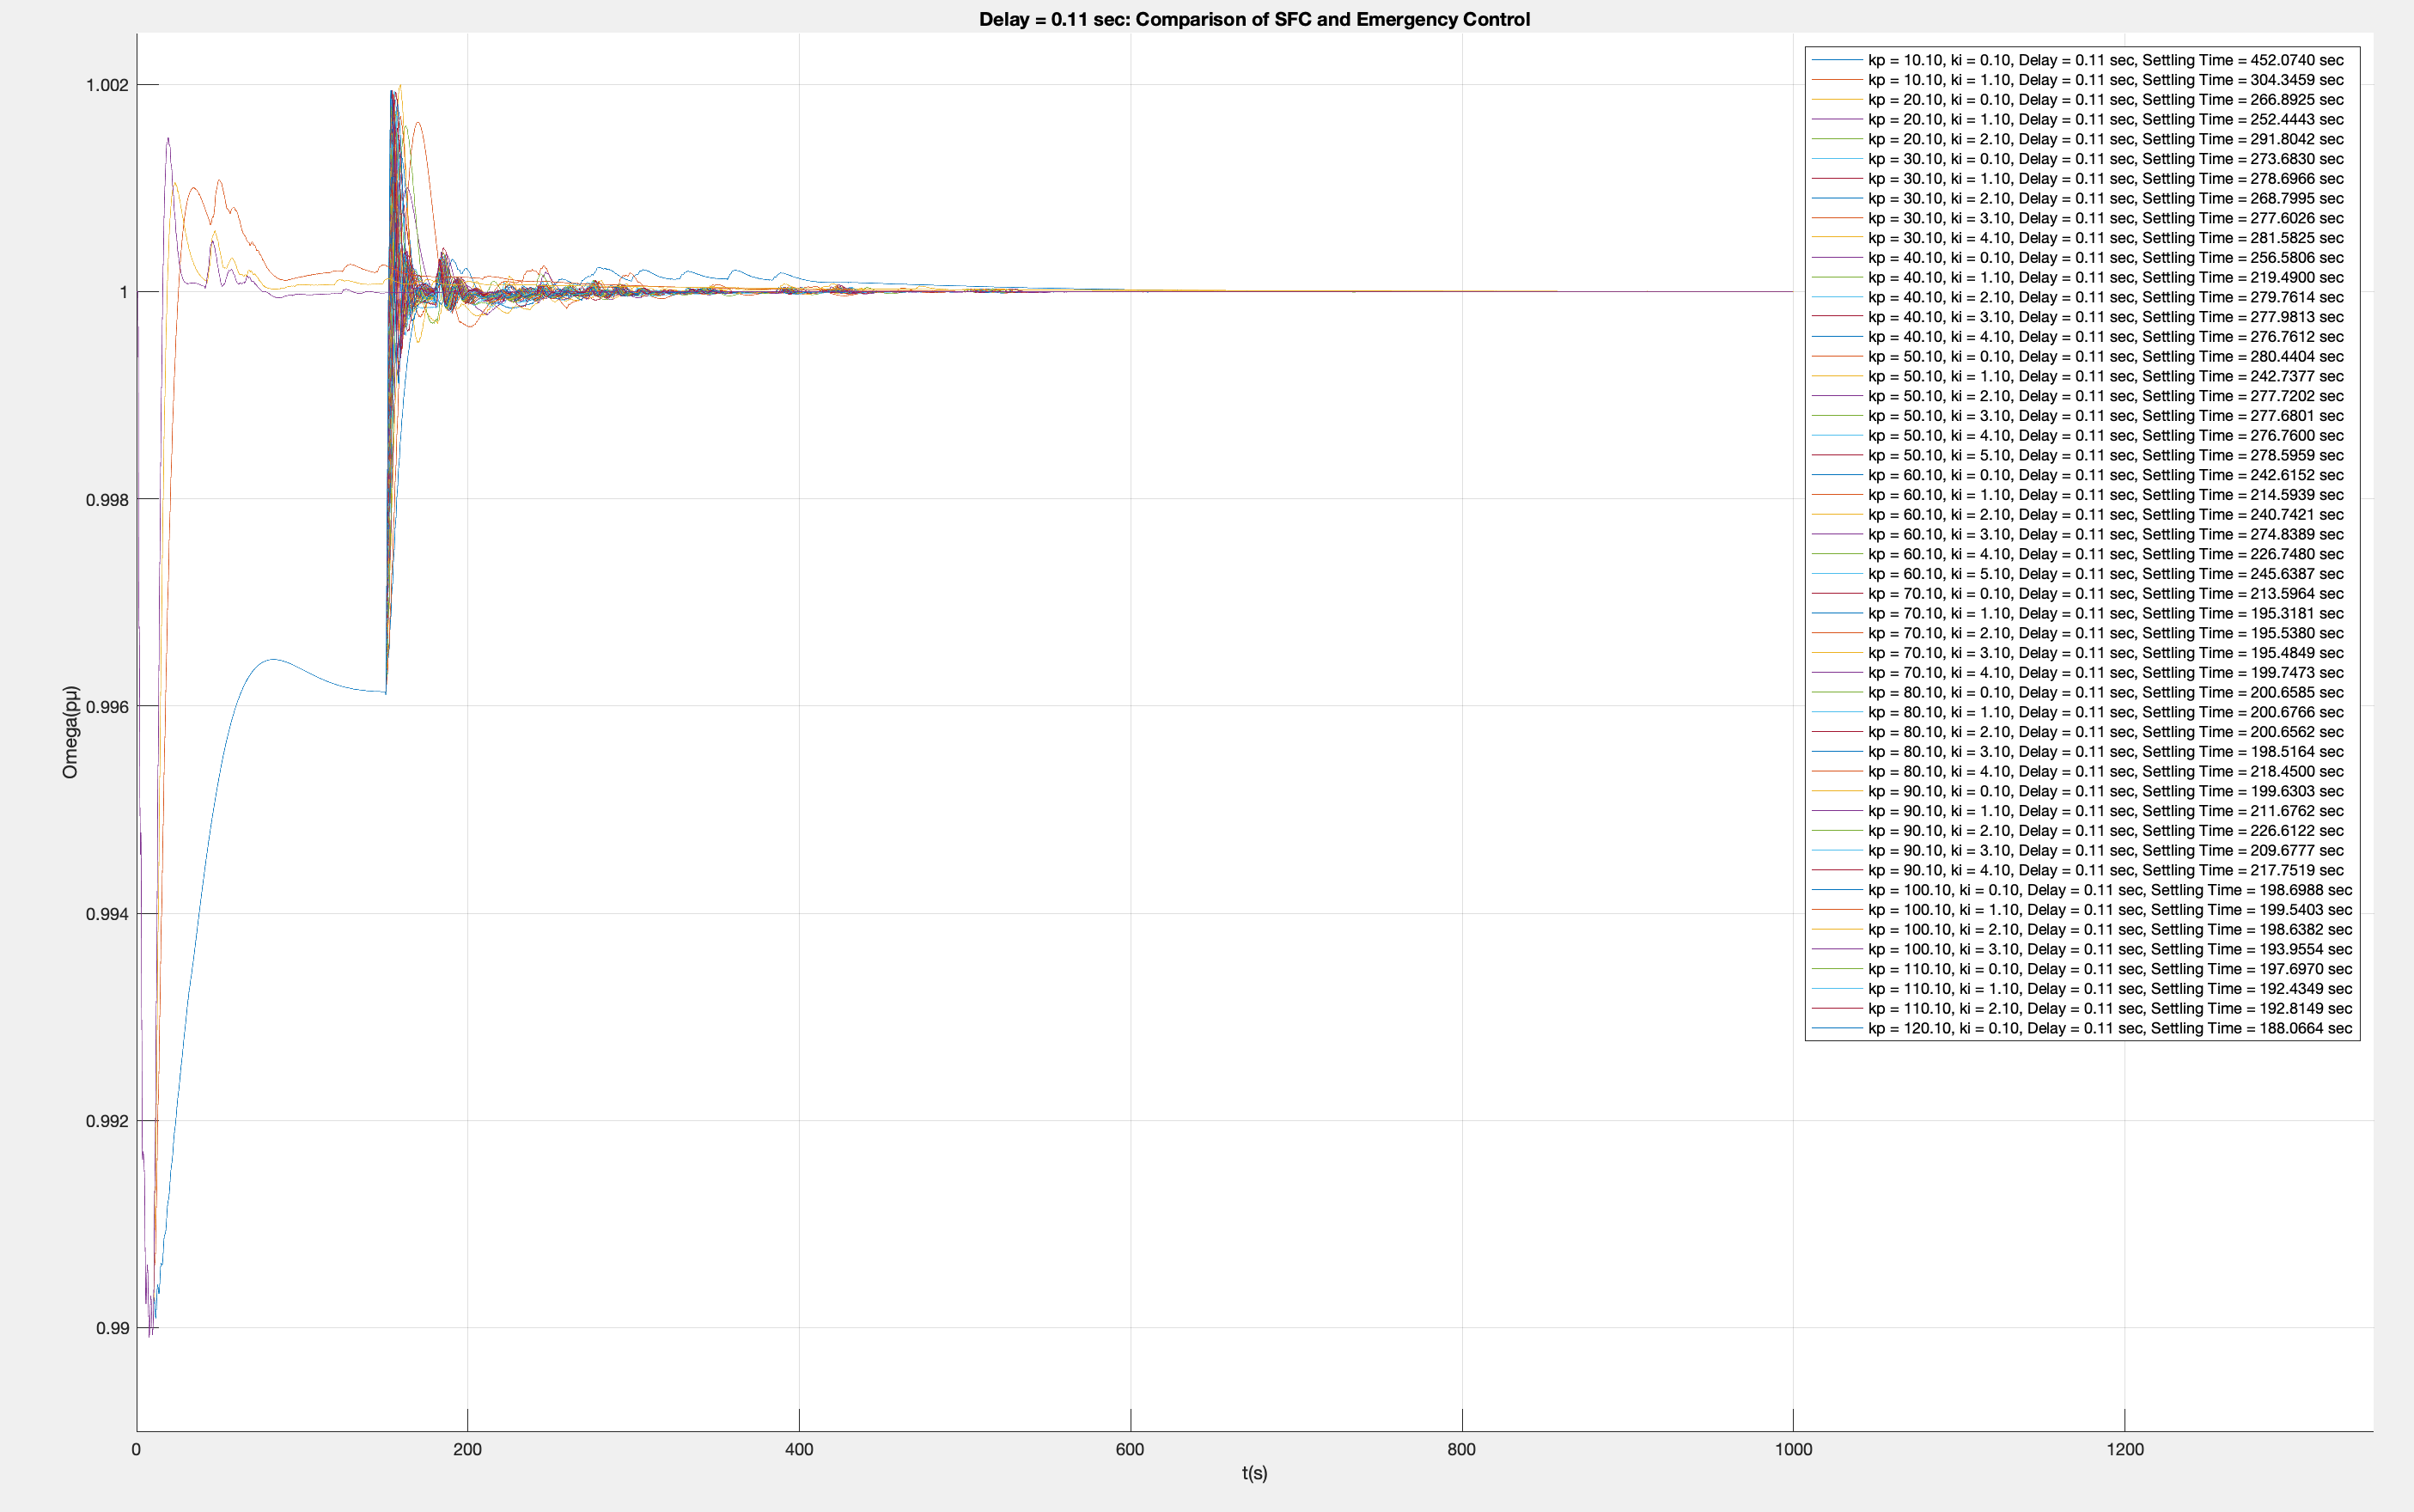
\includegraphics[width = .891\textwidth]{figure/6_4_CompaPlots_11.png}
\caption{Sketches for SFC and Emergency Control: Delay is 0.11 sec}
\label{6_4_CompaPlots_11}
\end{figure}


\begin{figure}[htbp]
\centering
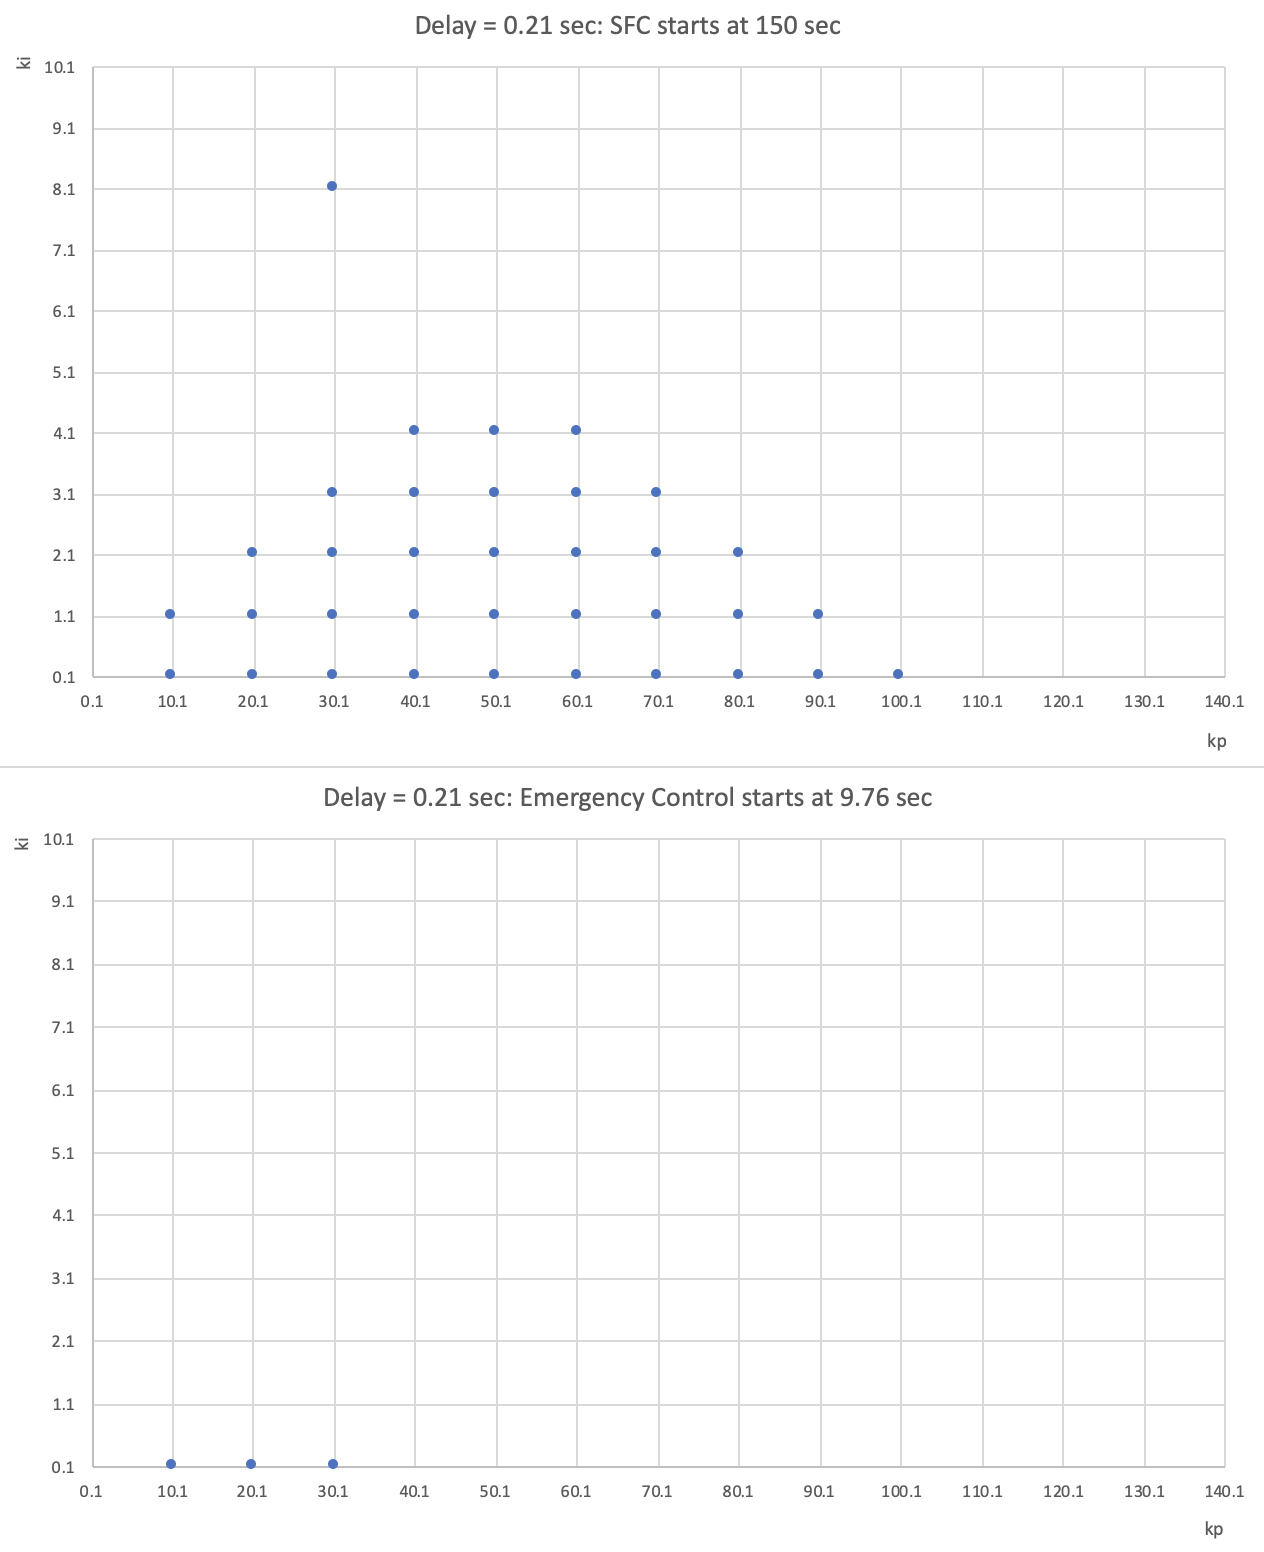
\includegraphics[width = .891\textwidth]{figure/6_4_copare_21.png}
\caption{Comparison: Delay is 0.21 sec}
\label{6_4_copare_21}
\end{figure}


\begin{figure}[htbp]
\centering
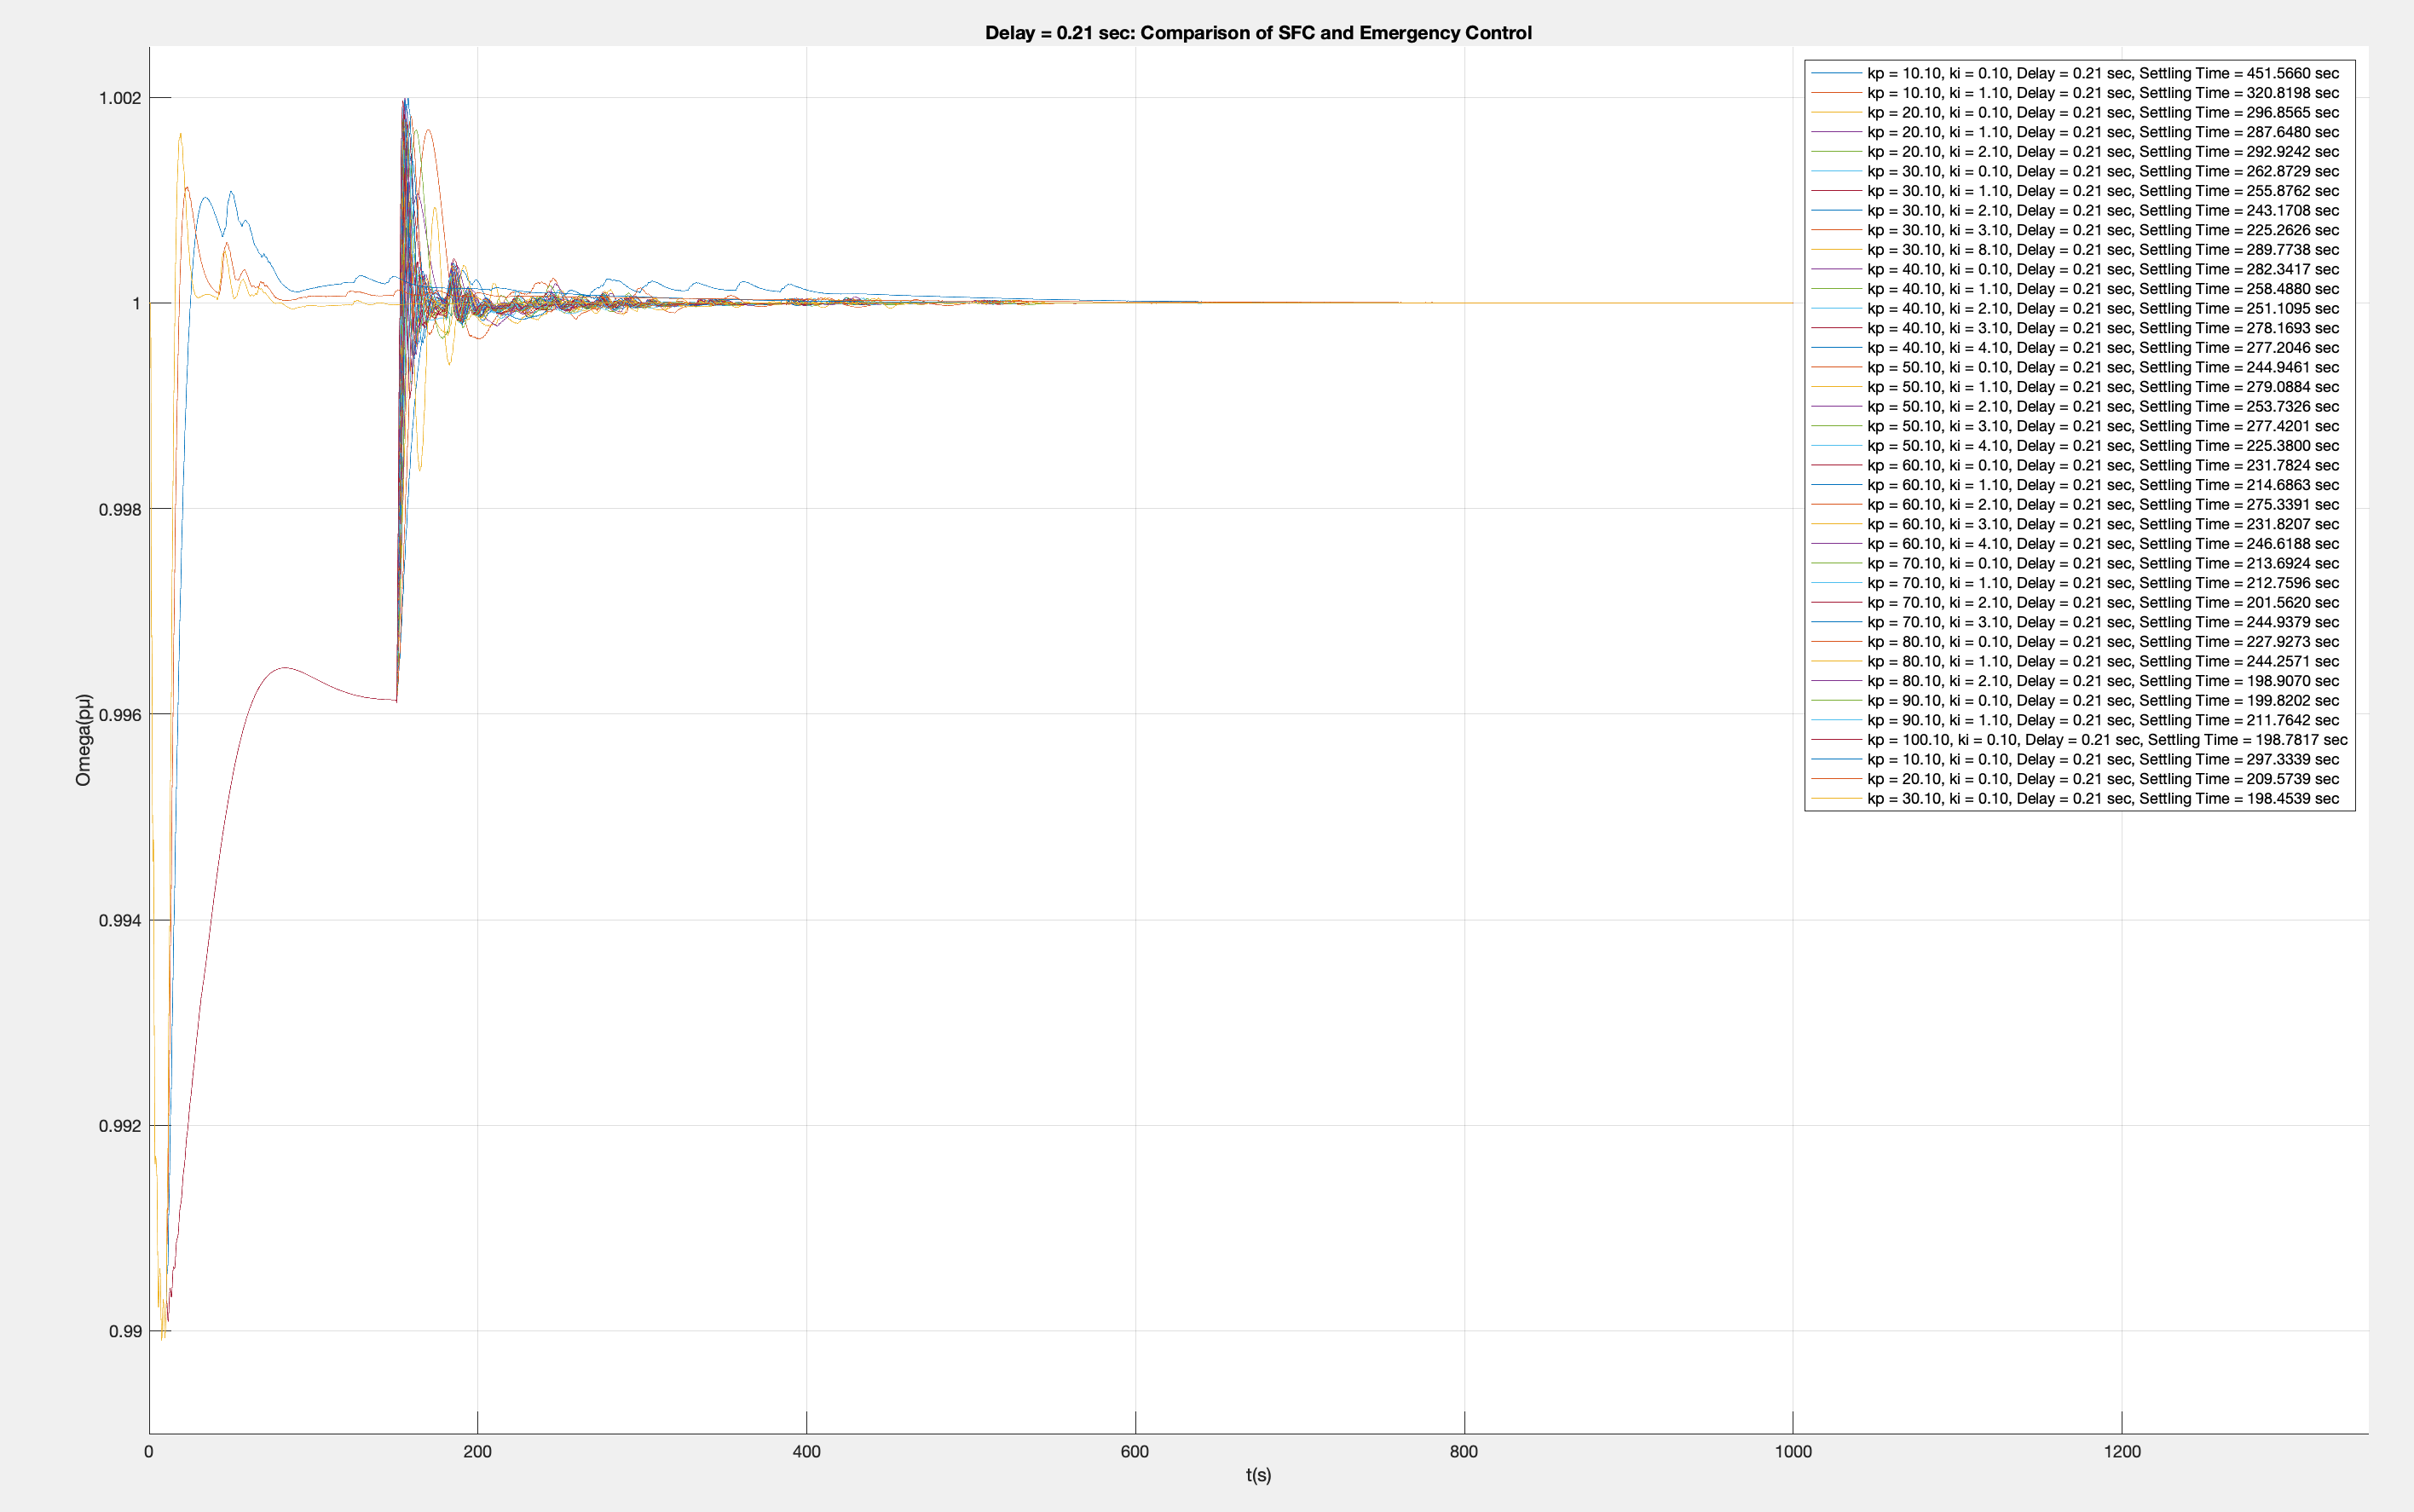
\includegraphics[width = .891\textwidth]{figure/6_4_CompaPlots_21.png}
\caption{Sketches for SFC and Emergency Control: Delay is 0.21 sec}
\label{6_4_CompaPlots_21}
\end{figure}




\subsection{The Best Tuning Result} %6.4.2
The best tuning result is compared with the signal without SFC control and is shown in Figure~\ref{6_4_2_best}.

\begin{figure}[htbp]
\centering
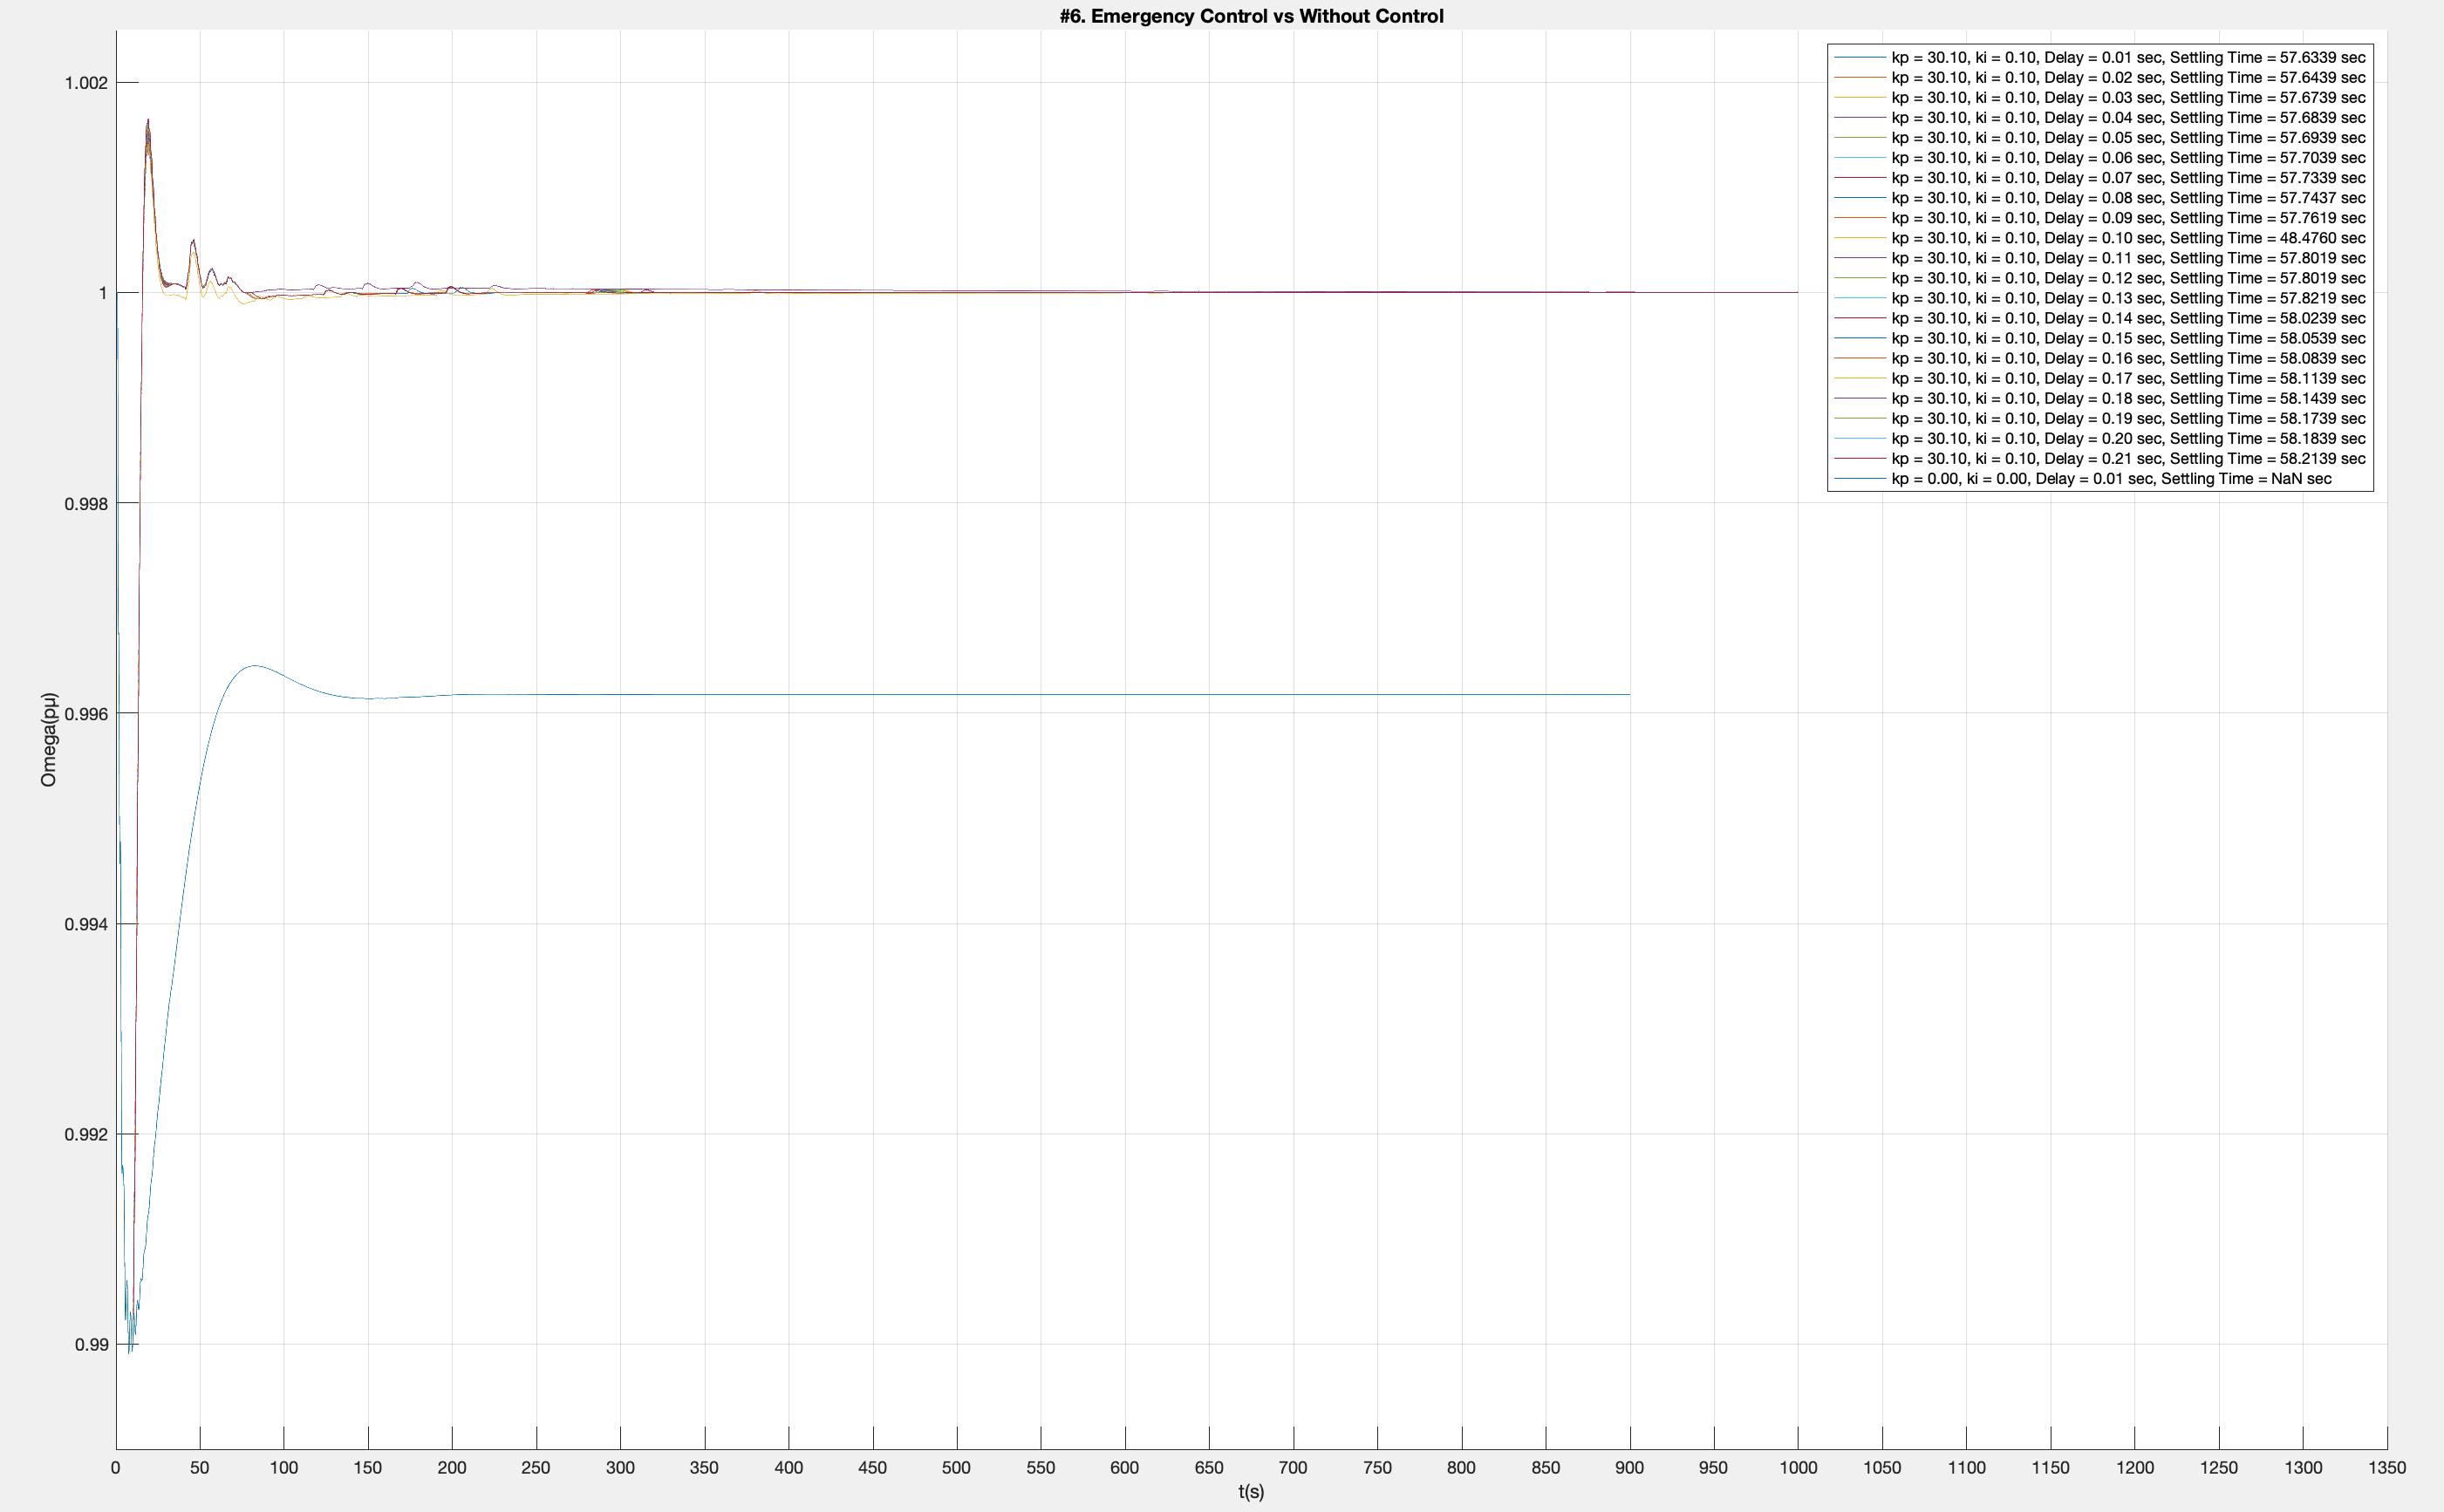
\includegraphics[width = .891\textwidth]{figure/6_4_2_best.png}
\caption{Best Emergency Control vs Without Control}
\label{6_4_2_best}
\end{figure}